% ============================================================
% Question Bank: ch03-06 Dividing Integers and Rational Numbers
% Topic Title: Dividing Integers and Rational Numbers
% CCSS: 7.NS.A.2
% Questions: 27 (15 MC + 6 SA + 6 Graphical)
% ============================================================

% --- Multiple Choice Questions (15) ---

\begin{practiceQuestion}{3-6-q01}{mc}
\begin{questionText}
What is $(-36) \div 6$?
\end{questionText}
\choiceA{$6$}
\choiceB{$-6$}
\choiceC{$-30$}
\choiceD{$30$}
\correctAnswer{B}
\explanation{Negative divided by positive is negative: $36 \div 6 = 6$, so $(-36) \div 6 = -6$.}
\end{practiceQuestion}

\begin{practiceQuestion}{3-6-q02}{mc}
\begin{questionText}
What is $(-48) \div (-8)$?
\end{questionText}
\choiceA{$-6$}
\choiceB{$6$}
\choiceC{$-40$}
\choiceD{$40$}
\correctAnswer{B}
\explanation{Negative divided by negative is positive: $48 \div 8 = 6$.}
\end{practiceQuestion}

\begin{practiceQuestion}{3-6-q03}{mc}
\begin{questionText}
What is $\dfrac{-15}{-3}$?
\end{questionText}
\choiceA{$-5$}
\choiceB{$5$}
\choiceC{$-12$}
\choiceD{$12$}
\correctAnswer{B}
\explanation{Both numerator and denominator are negative, so the quotient is positive: $15 \div 3 = 5$.}
\end{practiceQuestion}

\begin{practiceQuestion}{3-6-q04}{mc}
\begin{questionText}
A deep-sea probe descends $-240$ meters in $8$ minutes. What is the average rate of descent per minute?
\end{questionText}
\choiceA{$30$ m/min}
\choiceB{$-30$ m/min}
\choiceC{$-248$ m/min}
\choiceD{$-232$ m/min}
\correctAnswer{B}
\explanation{$(-240) \div 8 = -30$ m/min. The negative sign indicates descent.}
\end{practiceQuestion}

\begin{practiceQuestion}{3-6-q05}{mc}
\begin{questionText}
What is $0 \div (-9)$?
\end{questionText}
\choiceA{$0$}
\choiceB{$-9$}
\choiceC{$9$}
\choiceD{undefined}
\correctAnswer{A}
\explanation{Zero divided by any nonzero number is $0$: $0 \div (-9) = 0$.}
\end{practiceQuestion}

\begin{practiceQuestion}{3-6-q06}{mc}
\begin{questionText}
What is $(-7) \div 0$?
\end{questionText}
\choiceA{$0$}
\choiceB{$-7$}
\choiceC{$7$}
\choiceD{undefined}
\correctAnswer{D}
\explanation{Division by zero is undefined. You cannot divide any number by $0$.}
\end{practiceQuestion}

\begin{practiceQuestion}{3-6-q07}{mc}
\begin{questionText}
What is $\dfrac{-5}{6} \div \dfrac{2}{3}$?
\end{questionText}
\choiceA{$-\dfrac{5}{4}$}
\choiceB{$\dfrac{5}{4}$}
\choiceC{$-\dfrac{10}{18}$}
\choiceD{$-\dfrac{5}{9}$}
\correctAnswer{A}
\explanation{Multiply by the reciprocal: $\dfrac{-5}{6} \times \dfrac{3}{2} = \dfrac{-15}{12} = -\dfrac{5}{4}$.}
\end{practiceQuestion}

\begin{practiceQuestion}{3-6-q08}{mc}
\begin{questionText}
A football team loses $28$ yards in $4$ plays. What is the average yards per play?
\end{questionText}
\choiceA{$7$ yards}
\choiceB{$-7$ yards}
\choiceC{$24$ yards}
\choiceD{$-24$ yards}
\correctAnswer{B}
\explanation{$(-28) \div 4 = -7$ yards per play. The negative represents a loss.}
\end{practiceQuestion}

\begin{practiceQuestion}{3-6-q09}{mc}
\begin{questionText}
What is $-4.8 \div (-1.6)$?
\end{questionText}
\choiceA{$-3.0$}
\choiceB{$3.0$}
\choiceC{$-6.4$}
\choiceD{$6.4$}
\correctAnswer{B}
\explanation{Negative divided by negative is positive: $4.8 \div 1.6 = 3.0$.}
\end{practiceQuestion}

\begin{practiceQuestion}{3-6-q10}{mc}
\begin{questionText}
Which expression has the same value as $\dfrac{-18}{3}$?
\end{questionText}
\choiceA{$\dfrac{18}{3}$}
\choiceB{$\dfrac{18}{-3}$}
\choiceC{$\dfrac{-18}{-3}$}
\choiceD{$-\dfrac{18}{-3}$}
\correctAnswer{B}
\explanation{$\dfrac{-18}{3} = -6$. Choice B: $\dfrac{18}{-3} = -6$. A: $6$. C: $6$. D: $-\dfrac{18}{-3} = -(6) = -6$, but B is the standard equivalent form.}
\end{practiceQuestion}

\begin{practiceQuestion}{3-6-q11}{mc}
\begin{questionText}
What is $\left(-\dfrac{3}{8}\right) \div \left(-\dfrac{9}{16}\right)$?
\end{questionText}
\choiceA{$\dfrac{2}{3}$}
\choiceB{$-\dfrac{2}{3}$}
\choiceC{$\dfrac{27}{128}$}
\choiceD{$-\dfrac{27}{128}$}
\correctAnswer{A}
\explanation{Multiply by the reciprocal: $\dfrac{-3}{8} \times \dfrac{-16}{9} = \dfrac{48}{72} = \dfrac{2}{3}$. Two negatives make positive.}
\end{practiceQuestion}

\begin{practiceQuestion}{3-6-q12}{mc}
\begin{questionText}
If $x \div (-5) = 9$, what is $x$?
\end{questionText}
\choiceA{$45$}
\choiceB{$-45$}
\choiceC{$-14$}
\choiceD{$14$}
\correctAnswer{B}
\explanation{$x = 9 \times (-5) = -45$. Check: $(-45) \div (-5) = 9$. Correct.}
\end{practiceQuestion}

\begin{practiceQuestion}{3-6-q13}{mc}
\begin{questionText}
The temperature dropped $18°$F over $6$ hours. What was the average hourly change?
\end{questionText}
\choiceA{$3°$F per hour}
\choiceB{$-3°$F per hour}
\choiceC{$12°$F per hour}
\choiceD{$-12°$F per hour}
\correctAnswer{B}
\explanation{$(-18) \div 6 = -3°$F per hour. The temperature dropped an average of $3°$F each hour.}
\end{practiceQuestion}

\begin{practiceQuestion}{3-6-q14}{mc}
\begin{questionText}
What is $5.6 \div (-0.7)$?
\end{questionText}
\choiceA{$8$}
\choiceB{$-8$}
\choiceC{$0.8$}
\choiceD{$-0.8$}
\correctAnswer{B}
\explanation{Positive divided by negative is negative: $5.6 \div 0.7 = 8$, so the result is $-8$.}
\end{practiceQuestion}

\begin{practiceQuestion}{3-6-q15}{mc}
\begin{questionText}
Which has a negative quotient?
\end{questionText}
\choiceA{$(-24) \div (-6)$}
\choiceB{$36 \div 9$}
\choiceC{$(-32) \div 8$}
\choiceD{$0 \div (-5)$}
\correctAnswer{C}
\explanation{A: $+4$. B: $+4$. C: $(-32) \div 8 = -4$ (negative ÷ positive = negative). D: $0$.}
\end{practiceQuestion}

% --- Short Answer Questions (6) ---

\begin{practiceQuestion}{3-6-q16}{sa}
\begin{questionText}
What is $(-72) \div (-9)$?
\end{questionText}
\correctAnswer{$8$}
\explanation{Negative ÷ negative = positive: $72 \div 9 = 8$.}
\end{practiceQuestion}

\begin{practiceQuestion}{3-6-q17}{sa}
\begin{questionText}
What is $\dfrac{3}{4} \div \left(-\dfrac{1}{2}\right)$?
\end{questionText}
\correctAnswer{$-\dfrac{3}{2}$ or $-1\dfrac{1}{2}$}
\explanation{Multiply by the reciprocal: $\dfrac{3}{4} \times (-2) = -\dfrac{6}{4} = -\dfrac{3}{2}$. Positive ÷ negative = negative.}
\end{practiceQuestion}

\begin{practiceQuestion}{3-6-q18}{sa}
\begin{questionText}
An elevator goes down $54$ floors in $6$ equal trips. How many floors per trip?
\end{questionText}
\correctAnswer{$-9$ floors per trip}
\explanation{$(-54) \div 6 = -9$ floors per trip. Each trip moves $9$ floors down.}
\end{practiceQuestion}

\begin{practiceQuestion}{3-6-q19}{sa}
\begin{questionText}
What is $-6.3 \div 0.9$?
\end{questionText}
\correctAnswer{$-7$}
\explanation{$6.3 \div 0.9 = 7$. Negative ÷ positive = negative: $-7$.}
\end{practiceQuestion}

\begin{practiceQuestion}{3-6-q20}{sa}
\begin{questionText}
What is $\left(-\dfrac{2}{3}\right) \div \left(-\dfrac{4}{9}\right)$?
\end{questionText}
\correctAnswer{$\dfrac{3}{2}$ or $1\dfrac{1}{2}$}
\explanation{Multiply by reciprocal: $\dfrac{-2}{3} \times \dfrac{-9}{4} = \dfrac{18}{12} = \dfrac{3}{2}$. Two negatives = positive.}
\end{practiceQuestion}

\begin{practiceQuestion}{3-6-q21}{sa}
\begin{questionText}
A company lost $\$5{,}400$ over $3$ months. What was the average monthly loss?
\end{questionText}
\correctAnswer{$-\$1{,}800$ per month}
\explanation{$(-5{,}400) \div 3 = -1{,}800$. The company averaged $\$1{,}800$ loss per month.}
\end{practiceQuestion}

% --- Graphical Questions (3 GMC + 3 GSA) ---

\begin{practiceQuestion}{3-6-q22}{gmc}
\begin{questionText}
The diagram shows $-12$ split into equal groups. How many are in each group?

\begin{center}
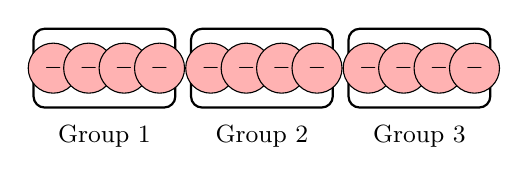
\begin{tikzpicture}[scale=0.5]
  \foreach \g in {0,4,8}{
    \draw[thick,rounded corners] (\g-0.3,-0.5) rectangle (\g+3.3,1.5);
    \foreach \i in {0,...,3}{
      \node[circle,draw,fill=red!30,minimum size=0.5cm,font=\footnotesize] at (\g+\i*0.9+0.2,0.5) {$-$};
    }}
  \node[below,font=\small] at (1.5,-0.7) {Group 1};
  \node[below,font=\small] at (5.5,-0.7) {Group 2};
  \node[below,font=\small] at (9.5,-0.7) {Group 3};
\end{tikzpicture}
\end{center}
\end{questionText}
\choiceA{$-3$}
\choiceB{$-4$}
\choiceC{$4$}
\choiceD{$3$}
\correctAnswer{B}
\explanation{$(-12) \div 3 = -4$. Each group contains $4$ negative chips, representing $-4$.}
\end{practiceQuestion}

\begin{practiceQuestion}{3-6-q23}{gmc}
\begin{questionText}
The table shows a car's position relative to a starting point at equal time intervals. What is the rate of change per interval?

\begin{center}
\begin{tabular}{|c|c|}
\hline
\textbf{Time (min)} & \textbf{Position (mi)} \\
\hline
$0$ & $0$ \\ \hline
$5$ & $-10$ \\ \hline
$10$ & $-20$ \\ \hline
$15$ & $-30$ \\ \hline
\end{tabular}
\end{center}
\end{questionText}
\choiceA{$-10$ mi per $5$ min}
\choiceB{$-2$ mi per min}
\choiceC{Both A and B}
\choiceD{$2$ mi per min}
\correctAnswer{C}
\explanation{$(-30) \div 15 = -2$ mi/min. Or per interval: $(-10) \div 1 = -10$ mi per $5$ min. Both are correct.}
\end{practiceQuestion}

\begin{practiceQuestion}{3-6-q24}{gmc}
\begin{questionText}
A thermometer shows the temperature dropped from $0°$C to $-20°$C. If the drop occurred equally over $4$ hours, what was the hourly change?

\begin{center}
\begin{tikzpicture}[scale=0.4]
  \draw[thick] (0,-6) -- (0,2);
  \draw[thick] (-0.3,0) -- (0.3,0) node[right,font=\small] {$0°$C};
  \draw[thick] (-0.3,-5) -- (0.3,-5) node[right,font=\small] {$-20°$C};
  \draw[thick,<->,funRed] (-0.8,0) -- (-0.8,-5) node[midway,left,font=\small] {?/hr};
\end{tikzpicture}
\end{center}
\end{questionText}
\choiceA{$-4°$C/hr}
\choiceB{$-5°$C/hr}
\choiceC{$4°$C/hr}
\choiceD{$5°$C/hr}
\correctAnswer{B}
\explanation{$(-20) \div 4 = -5°$C per hour. The temperature fell $5°$C each hour.}
\end{practiceQuestion}

\begin{practiceQuestion}{3-6-q25}{gsa}
\begin{questionText}
The number line shows $-16$ being divided into equal jumps from $0$ to $-16$. Each jump is $-4$. How many jumps are there?

\begin{center}
\begin{tikzpicture}
  \draw[thick,->] (-17.5,0) -- (1.5,0);
  \foreach \x in {-16,-12,-8,-4,0} \draw (\x,0.1) -- (\x,-0.1) node[below,font=\small] {$\x$};
  \draw[thick,->,funBlue] (0,0.4) to[bend left=30] (-4,0.4);
  \draw[thick,->,funBlue] (-4,0.4) to[bend left=30] (-8,0.4);
  \draw[thick,->,funBlue] (-8,0.4) to[bend left=30] (-12,0.4);
  \draw[thick,->,funBlue] (-12,0.4) to[bend left=30] (-16,0.4);
\end{tikzpicture}
\end{center}
\end{questionText}
\correctAnswer{$4$ jumps}
\explanation{$(-16) \div (-4) = 4$ jumps. Four jumps of $-4$ go from $0$ to $-16$.}
\end{practiceQuestion}

\begin{practiceQuestion}{3-6-q26}{gsa}
\begin{questionText}
Complete the division table. What is the missing value?

\begin{center}
\begin{tabular}{|c|c|c|}
\hline
$a$ & $b$ & $a \div b$ \\
\hline
$20$ & $-4$ & $-5$ \\ \hline
$-20$ & $4$ & $-5$ \\ \hline
$-20$ & $-4$ & ? \\ \hline
\end{tabular}
\end{center}
\end{questionText}
\correctAnswer{$5$}
\explanation{$(-20) \div (-4) = 5$. Negative ÷ negative = positive. Same magnitude $20 \div 4 = 5$.}
\end{practiceQuestion}

\begin{practiceQuestion}{3-6-q27}{gsa}
\begin{questionText}
The bar graph shows Quiz $1$ through Quiz $4$ score changes. If a student's total score change was $-24$ points over the $4$ quizzes, what was the average change per quiz?

\begin{center}
\begin{tikzpicture}[scale=0.6]
  \draw[thick,->] (0,-4) -- (0,2);
  \draw[thick,->] (0,0) -- (5.5,0);
  \foreach \y in {-3,...,1} \draw (-0.15,\y) -- (0.15,\y) node[left=3pt,font=\footnotesize] {$\y$0};
  \draw (-0.15,0) node[left=3pt,font=\footnotesize] {$0$};
  \fill[funRed] (0.5,0) rectangle (1.2,-2);
  \fill[funGreen] (1.7,0) rectangle (2.4,1);
  \fill[funRed] (2.9,0) rectangle (3.6,-3);
  \fill[funGreen] (4.1,0) rectangle (4.8,0);
  \node[below,font=\footnotesize] at (0.85,0) {Q1};
  \node[below,font=\footnotesize] at (2.05,0) {Q2};
  \node[below,font=\footnotesize] at (3.25,0) {Q3};
  \node[below,font=\footnotesize] at (4.45,0) {Q4};
\end{tikzpicture}
\end{center}
\end{questionText}
\correctAnswer{$-6$ points per quiz}
\explanation{$(-24) \div 4 = -6$ points per quiz. The student lost an average of $6$ points per quiz.}
\end{practiceQuestion}
